\chapter{Metric spaces}
This chapter draws heavily from the first two lectures of \href{https://web.mit.edu/paigeb/www/18.S097/}{Introduction to Metric Spaces} taught by Paige Dote at MIT in 2022.

% ==================================================================================================

\section{Definition}
In the previous chapters, we used absolute value bars extensively to denote the distance between two real numbers. There are a few properties that make them intuitive and natural when quantifying distance. For all $x, y \in \R$,
\begin{itemize}
  \item $\abs{x - y} \geq 0$. Distances should be non-negative! Also, $\abs{x - y} = 0 \iff x = y$.
  \item $\abs{x - y} = \abs{x - y}$. The distance between $x$ and $y$ should be equal to the distance between $y$ and $x$.
  \item Triangle inequality: $\abs{x - z} \leq \abs{x - y} + \abs{y - z}$. This comes naturally from the definition of the absolute value bars, and we seemingly take this for granted when proving things in $\R$.
\end{itemize}

Metric spaces generalise this concept of distance to arbitrary sets.

\begin{definition}[Metric space]
  A metric space is a set $X$ with a metric $d: X \times X \to \R$ such that for all $x, y, z \in X$, the metric $d$ satisfies the following properties:
  \begin{itemize}
    \item Positive definite: 1) $d(x, y) \geq 0$ and 2) $d(x, y) = 0 \iff x = y$
    \item Symmetric: $d(x, y) = d(y, x)$
    \item Triangle inequality: $d(x, z) \leq d(x, y) + d(y, z)$
  \end{itemize}
\end{definition}
Positive definiteness restricts the codomain of $d$ to $[0, \infty)$, so we can write $d: X \times X \to [0, \infty)$ instead.

% ==================================================================================================

\section{Common metrics in $\R ^ n$}
We will now look at some common metrics.
\begin{definition}[Supremum metric]
  The supremum metric $d_{\infty}: \R ^ n \times \R ^ n \to [0, \infty)$ is defined by
  \[
    d_{\infty} (x, y) = \max_{1 \leq i \leq n} \abs{x_i - y_i}
  \]
\end{definition}
We check that it is a metric.
\begin{itemize}
  \item Positive definite: 
    \begin{itemize}
      \item Clearly, for all $i$, $\abs{x_i - y_i} \geq 0$, so $d_{\infty} (x, y) \geq 0$. 
      \item $d_{\infty} (x, y) = 0 \iff \abs{x_i - y_i} = 0$ for all $i \iff x = y$.
    \end{itemize}
  \item Symmetry: $d_{\infty} (x, y) = \max \abs{x_i - y_i} = \max \abs{y_i - x_i} = d_{\infty} (y, x)$. This follows immediately from the symmetry of absolute value bars.
  \item Triangle inequality: 
    \begin{align*}
      \begin{aligned}
        d_{\infty} (x, z) &= \max \abs{x_i - z_i} &&\quad \text{(attained at some $i_0$)} \\
        &\leq \max (\abs{x_i - y_i} + \abs{y_i - z_i}) &&\quad \text{holds for $i_0$, so holds for all $i$} \\
        &\leq \max \abs{x_i - y_i} + \max \abs{y_i - z_i} &&\quad \text{may not be attained at same $i$} \\
        &= d_{\infty} (x, y) + d_{\infty} (y, z).
      \end{aligned}
    \end{align*} 
    This follows from the triangle inequality for absolute value bars.
\end{itemize}

\begin{definition}[$\ell ^ 1$ metric]
  The $\ell ^ 1$ metric $d_1: \R ^ n \times \R ^ n \to [0, \infty)$ is defined by
  \[
    d_1 (x, y) = \sum_{i = 1} ^ {n} \abs{x_i - y_i}
  \]
\end{definition}
We check that it is a metric.
\begin{itemize}
  \item Positive definite:
    \begin{itemize}
      \item Clearly, for all $i$, $\abs{x_i - y_i} \geq 0$, so their sum also $\geq 0$, and $d_1 (x, y) \geq 0$.
      \item $d_1 (x, y) = 0 \iff \sum \abs{x_i - y_i} = 0 \iff x_i = y_i$ for all $i \iff x = y$.
    \end{itemize}
  \item Symmetry: 
    \[
      d_1 (x, y) = \sum \abs{x_i - y_i} = \sum \abs{y_i - x_i} = d_1 (y, x).
    \]
  \item Triangle inequality:
    \begin{align*}
      \begin{aligned}
        d_1 (x, z) &= \sum \abs{x_i - z_i} \\ 
        &\leq \sum \abs{x_i - y_i} + \abs{y_i - z_i} \\ 
        &= \sum \abs{x_i - y_i} + \sum \abs{y_i - z_i} &&\quad \text{by linearity of summation} \\
        &= d_1 (x, y) + d_1 (y, z)
      \end{aligned}
    \end{align*}
\end{itemize}

Now, we will consider the set of continuous functions $C ^ 0 ([a, b])$, where every element is a function of type $[a, b] \to \R$ which is continuous on $[a, b]$.
\begin{eg}
  Show that $d: C ^ 0 ([0, 1]) \times C ^ 0 ([0, 1]) \to [0, \infty)$ defined by
  \[
    d(f, g) = \sup_{x \in [0, 1]} \abs{f(x) - g(x)}
  \]
  is a metric.
\end{eg}
\begin{solution}
  Positive definiteness and symmetry are straightforward. For triangle inequality, take arbitrary $f, h \in C ^ 0 ([0, 1])$. Since $f$ and $h$ are both continuous on a closed interval $[0, 1]$, the function $\abs{f(x) - h(x)}$ is also continuous on $[0, 1]$. By the Extreme Value Theorem, there exists $x_0$ such that
  \[
    \abs{f(x_0) - h(x_0)} = \sup_{x \in [0, 1]} \abs{f(x) - h(x)}
  \]
  Then we have
  \begin{align*}
    \begin{aligned}
      d(f, h) &= \sup_{x \in [0, 1]} \abs{f(x) - h(x)} \\ 
      &= \abs{f(x_0) - h(x_0)} \\ 
      &\leq \abs{f(x_0) - g(x_0)} + \abs{g(x_0) - h(x_0)} &&\quad \text{by $\triangle$} \\
      &\leq \sup_{x \in [0, 1]} \abs{f(x) - g(x)} + \sup_{x \in [0, 1]} \abs{g(x) - h(x)}  &&\quad \text{by definition of supremum} \\
      &= d(f, g) + d(g, h)
    \end{aligned}
  \end{align*}
\end{solution}
Next, we consider the set of continuously differentiable functions $C ^ 1 ([a, b])$.
\begin{eg}
  Show that $d: C ^ 1 ([0, 1]) \times C ^ 1 ([0, 1]) \to [0, \infty)$ defined by
  \[
    d(f, g) = \sup_{x \in [0, 1]} \abs{f(x) - g(x)} + \sup_{x \in [0, 1]} \abs{f'(x) - g'(x)}
  \]
  is a metric.
\end{eg}
\begin{solution}
  For triangle inequality, from the above example, we know that
  \[
    \sup_{x \in [0, 1]} \abs{f(x) - h(x)} \leq \sup_{x \in [0, 1]} \abs{f(x) - g(x)} + \sup_{x \in [0, 1]} \abs{g(x) - h(x)}
  \]
  since $f, g, h \in C ^ 0 ([0, 1])$ as well (they are all continuous on $[0, 1]$). Also, their derivatives $f', g', h' \in C ^ 0 ([0, 1])$ by definition, so
  \[
    \sup_{x \in [0, 1]} \abs{f'(x) - h'(x)} \leq \sup_{x \in [0, 1]} \abs{f'(x) - g'(x)} + \sup_{x \in [0, 1]} \abs{g'(x) - h'(x)}
  \]
  We add the two inequalities and we are done.
\end{solution}
\begin{eg}[PSET 1 Q2]
  Is $d: C ^ 1 ([0, 1]) \times C ^ 1 ([0, 1]) \to [0, \infty)$ defined by
  \[
    d(f, g) = \sup_{x \in [0, 1]} \abs{f'(x) - g'(x)}
  \]
  a metric on $C ^ 1 ([0, 1])$? If so, prove it. If not, show what properties of a metric $d$ satisfies, and explain which properties of a metric $d$ fails.
\end{eg}
\begin{solution}
  \ \newline
  \begin{itemize}
    \item Positive definite:
      \begin{itemize}
        \item Clearly, $d(f, g) \geq 0$ for all $f, g \in C ^ 1 ([0, 1])$.
        \item If $f = g$, then $f'(x) - g'(x) = 0$ for all $x \in [0, 1]$, so $d(f, g) = 0$. However, if $d(f, g) = 0$, we get $f'(x) = g'(x)$ for all $x \in [0, 1]$, but this does not imply $f = g$. For instance, take $f(x) = x$ and $g(x) = x + 1$.
      \end{itemize}
      Therefore, $d$ is not positive definite.
    \item Symmetry: follows from absolute value bars.
    \item Triangle inequality: similar to a previous example with $C ^ 0 ([0, 1])$.
  \end{itemize}
\end{solution}
\begin{eg}
  Let $(X, d)$ be a metric space. Show that $\tilde{d}: X \times X \to [0, \infty)$ defined by
  \[
    \tilde{d}(x, y) = \frac{d(x, y)}{1 + d(x, y)} 
  \]
  is a metric, and show that $X$ is bounded in the metric $\tilde{d}$.
\end{eg}
\begin{solution}
  \ \newline
  \begin{itemize}
    \item Positive definite:
      \begin{itemize}
        \item Since $d(x, y) \geq 0$ and $1 + d(x, y) \geq 0$, $\tilde{d}(x, y) \geq 0$.
        \item $\tilde{d}(x, y) = 0 \iff d(x, y) = 0 \iff x = y$.
      \end{itemize}
    \item Symmetry:
      \[
        \tilde{d}(x, y) = \frac{d(x, y)}{1 + d(x, y)} = \frac{d(y, x)}{1 + d(y, x)} = \tilde{d}(y, x) 
      \]
    \item Triangle inequality:
      \begin{align*}
        \tilde{d}(x, z) &= \frac{d(x, z)}{1 + d(x, z)} \\ 
        &= 1 - \frac{1}{1 + d(x, z)} \\ 
        &\leq 1 - \frac{1}{1 + d(x, y) + d(y, z)} \\ 
        &= \frac{d(x, y) + d(y, z)}{1 + d(x, y) + d(y, z)} \\ 
        &= \frac{d(x, y)}{1 + d(x, y) + d(y, z)} + \frac{d(y, z)}{1 + d(x, y) + d(y, z)} \\
        &\leq \frac{d(x, y)}{1 + d(x, y)} + \frac{d(y, z)}{1 + d(y, z)} \\
        &= \tilde{d}(x, y) + \tilde{d}(y, z)
      \end{align*}
  \end{itemize}

  Fix any $x \in X$. For every $y \in X$, $\tilde{d}(x, y) < 1$, so $X$ is bounded in $\tilde{d}$.
\end{solution}
\begin{eg}
  Show that the map $\frac{\di}{\di x}: C ^ 1 ([a, b]) \to C ^ 0 ([a, b])$ is continuous with respect to the uniform distance.
\end{eg}
\begin{solution}
  Take arbitrary $f, g \in C ^ 1 ([a, b])$. We want to show that 
  \[
    \forall \epsilon > 0, \; \exists \delta > 0: 0 < d_{C ^ 1}(f, g) < \delta \implies d_{C ^ 0}(\frac{\di}{\di x} f, \frac{\di}{\di x} g) < \epsilon
  \]
  By definition,
  \[
    d_{C ^ 1}(f, g) = \sup_{x \in [a, b]} \abs{f(x) - g(x)} + \sup_{x \in [a, b]} \abs{f'(x) - g'(x)}
  \]
  and
  \[
    d_{C ^ 0}(f', g') = \sup_{x \in [a, b]} \abs{f'(x) - g'(x)} 
  \]
  Observe that $d_{C ^ 0}(f', g') \leq d_{C ^ 1}(f, g)$, so set $\delta = \epsilon$.
\end{solution}
\begin{eg}[PSET 1 Q5]
  Show that the map $I_t: C ^ 0 ([a, b]) \to C ^ 1 ([a, b])$ is continuous, where
  \[
    I_x(f) = \int_{a}^{x} \! f(t) \di t
  \]
  Assume we are using the uniform distances for $C ^ 0 ([a, b])$ and $C ^ 1 ([a, b])$ as metrics.
\end{eg}
\begin{solution}
   Take arbitrary $f, g \in C ^ 0 ([a, b])$. We want to show that
  \[
    \forall \epsilon > 0, \; \exists \delta > 0: 0 < d_{C ^ 0}(f, g) < \delta \implies d_{C ^ 1}(I_x(f), I_x(g)) < \epsilon
  \]
  As usual, we start from the consequent:
  \begin{align*}
    \begin{aligned}
      d_{C ^ 1}(I_x(f), I_x(g)) &= \sup_{x \in [a, b]} \abs{I_x(f) - I_x(g)} + \sup_{x \in [a, b]} \abs{f(x) - g(x)} \\ 
      &= \sup_{x \in [a, b]} \abs{\int_a^x f(t) \! \di t - \int_a^x g(t) \! \di t} + \sup_{x \in [a, b]} \abs{f(x) - g(x)} \\ 
      &= \sup_{x \in [a, b]} \abs{\int_a^x f(t) - g(t) \! \di t} + \sup_{x \in [a, b]} \abs{f(x) - g(x)} &&\quad \text{by linearity of integration} \\
      &\leq \sup_{x \in [a, b]} \int_a^x \abs{f(t) - g(t)} \! \di t + \sup_{x \in [a, b]} \abs{f(x) - g(x)} &&\quad \text{by analogue version of $\triangle$} \\ 
      &\leq (b - a) \sup_{x \in [a, b]} \abs{f(x) - g(x)} + \sup_{x \in [a, b]} \abs{f(x) - g(x)} &&\quad \text{refer to \Cref{fig:week_09_int}} \\ 
      &= (1 + b - a) \sup_{x \in [a, b]} \abs{f(x) - g(x)} \\ 
      &< \epsilon
    \end{aligned}
  \end{align*}
  So we pick $\displaystyle \delta = \frac{\epsilon}{1 + b - a}$.
\end{solution}
\begin{figure}
  \centering
  \begin{minipage}{.4\textwidth}
    \centering
    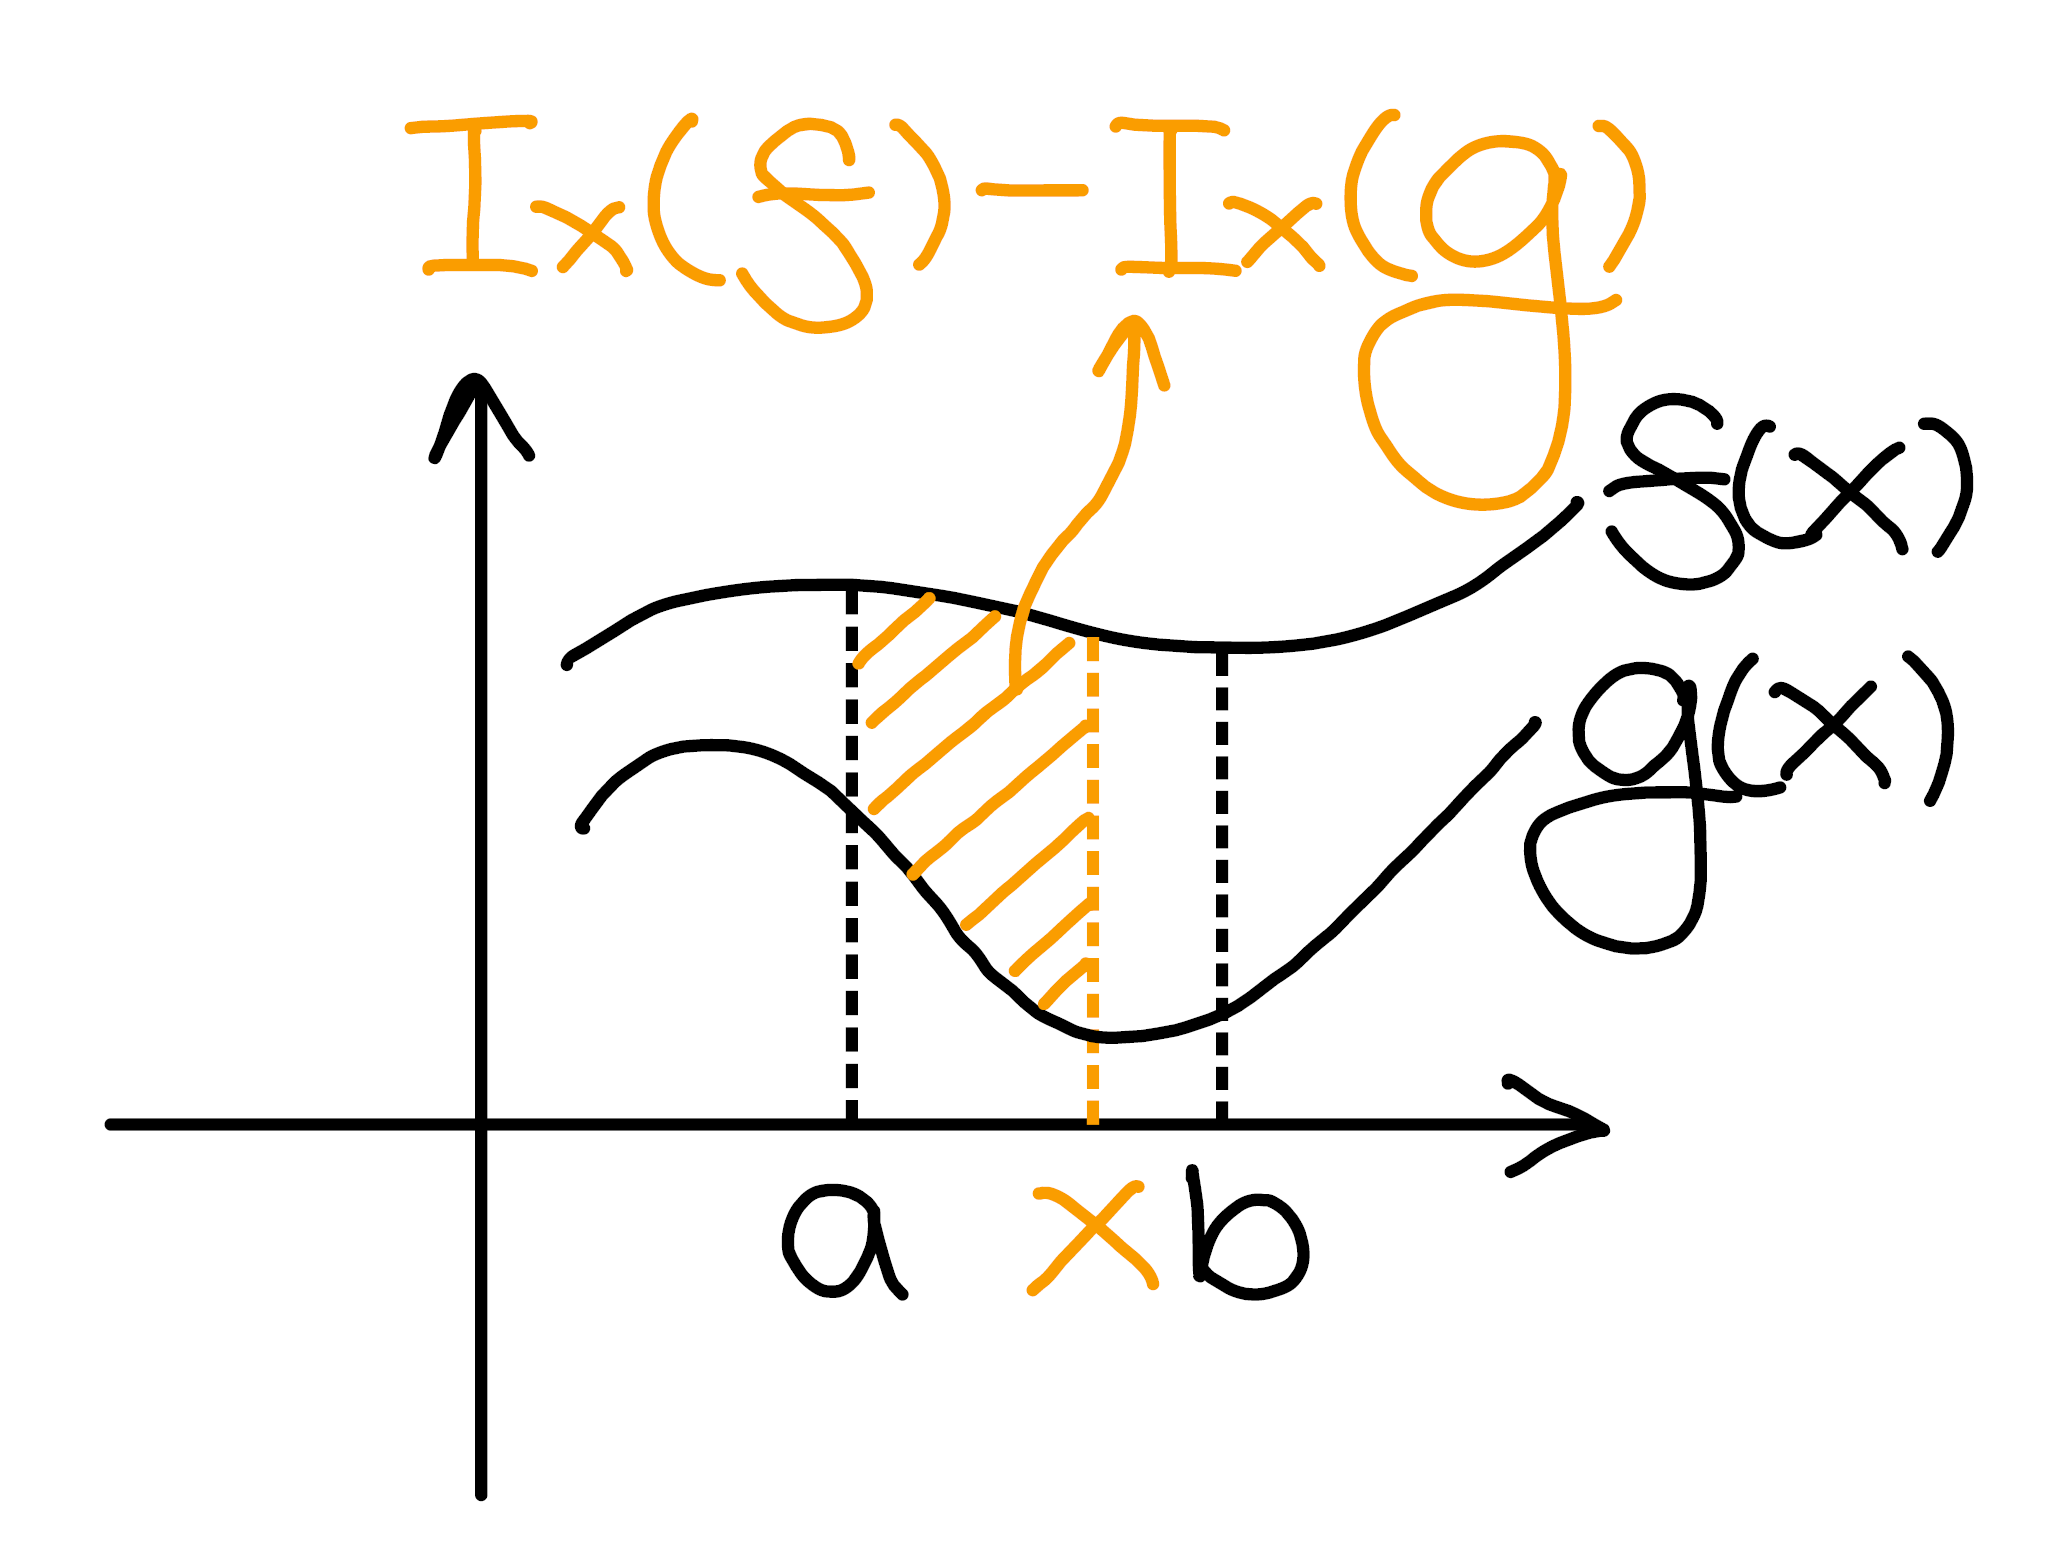
\includegraphics[width=\linewidth]{week_09_int_1}
    % \label{fig:week_09_int_1}
  \end{minipage}%
  \begin{minipage}{.6\textwidth}
    \centering
    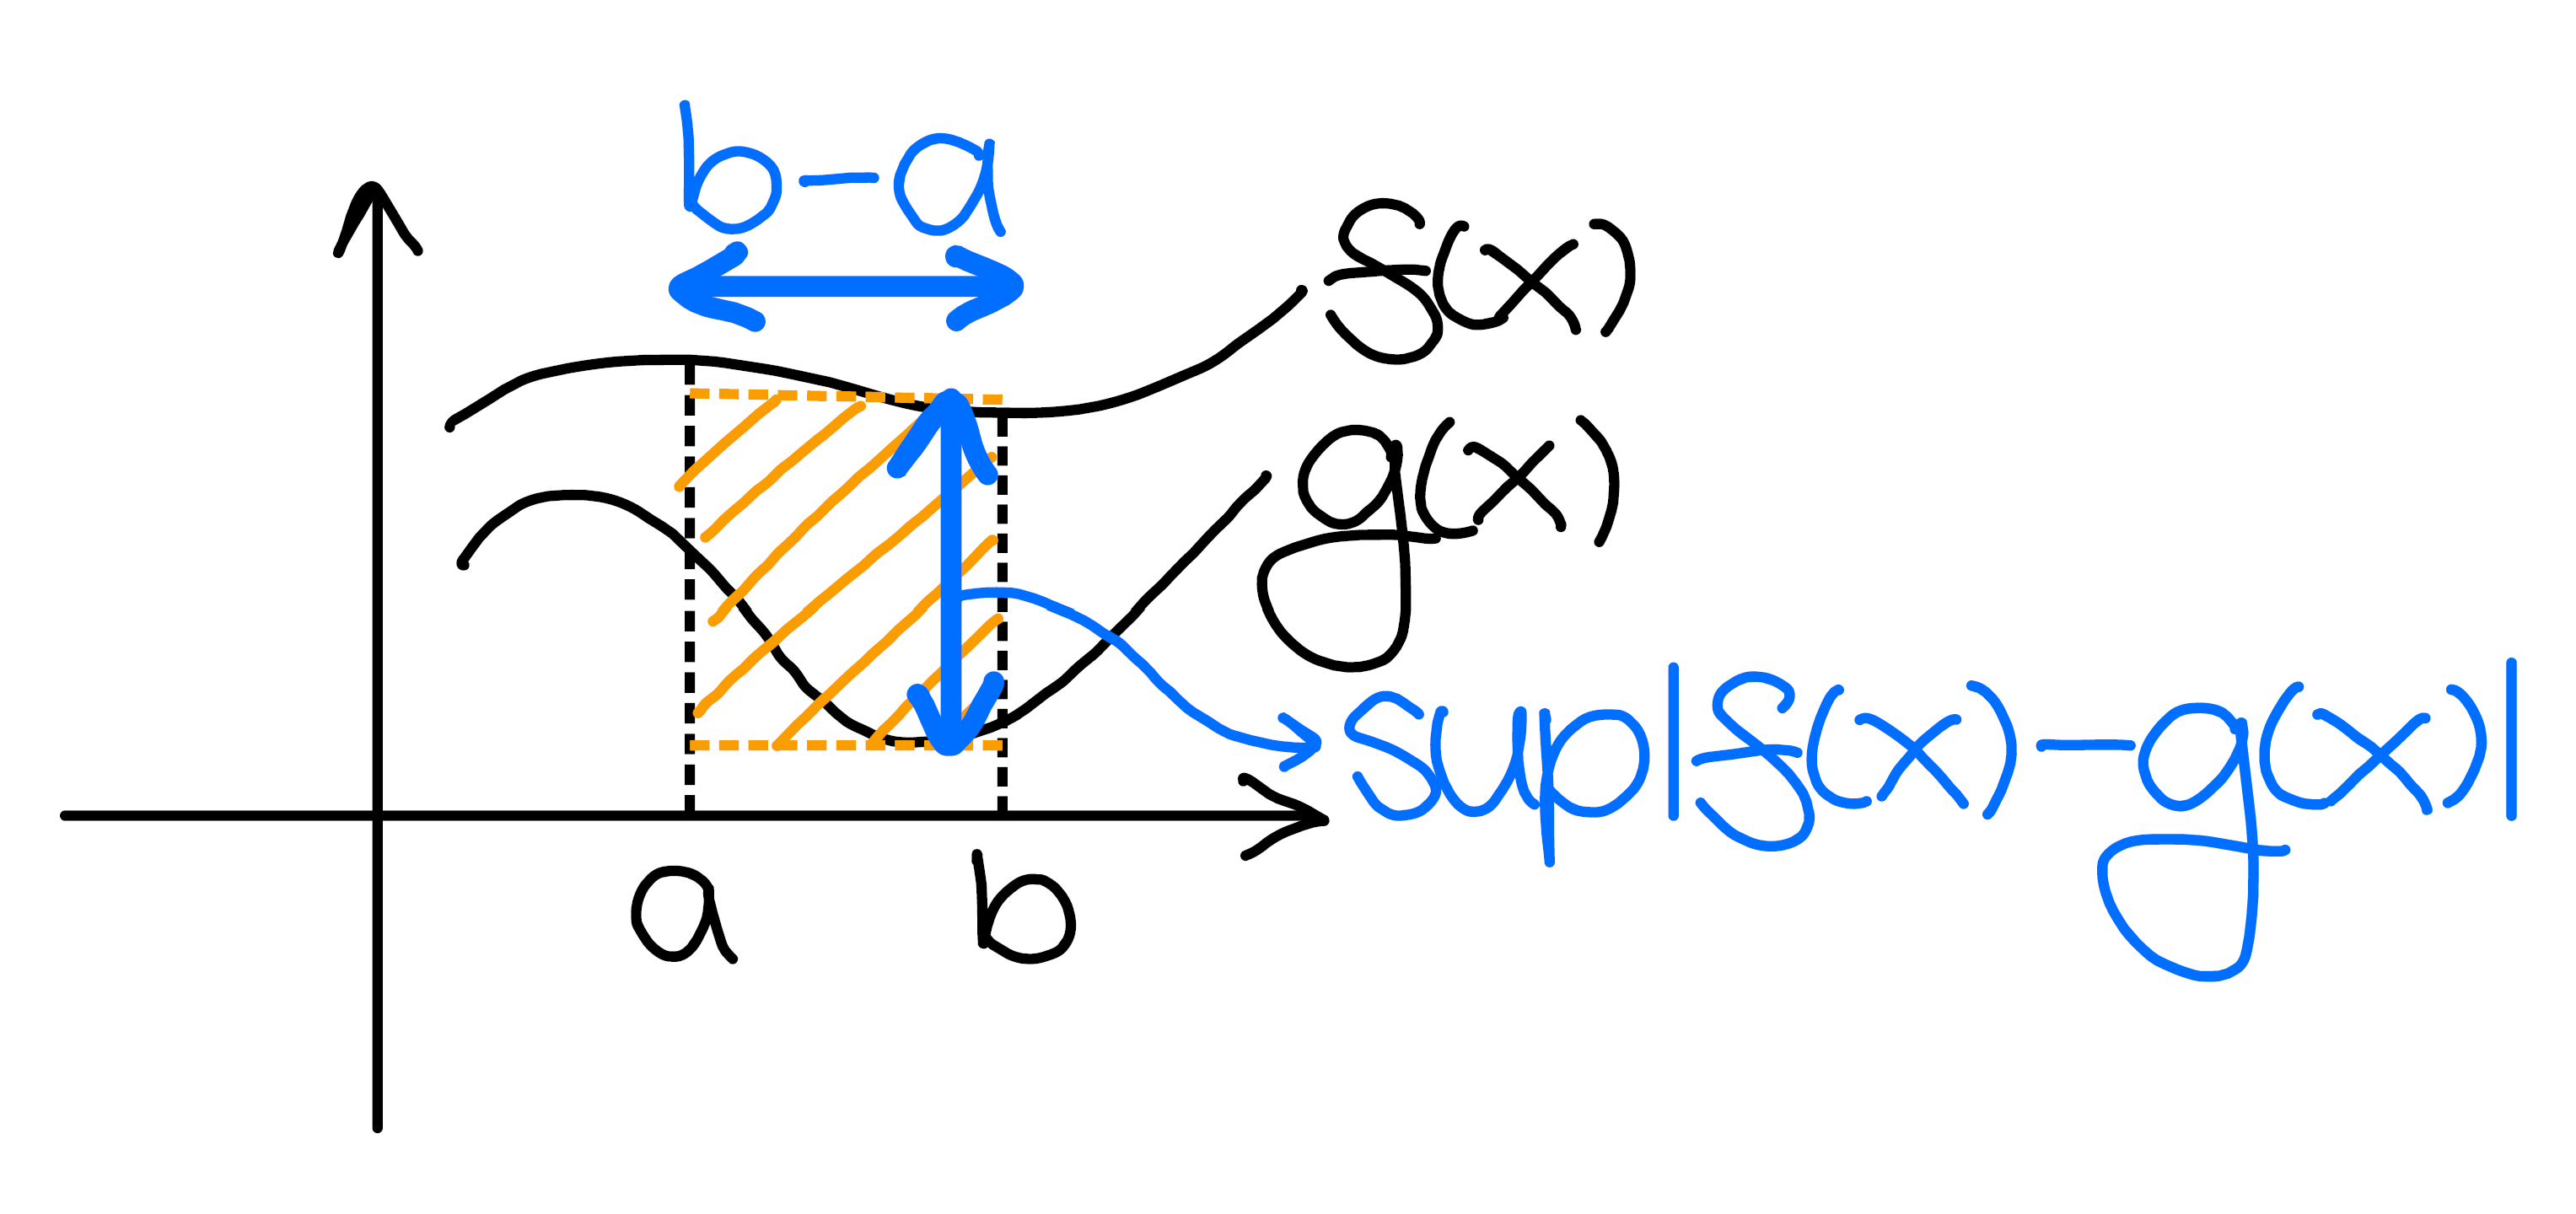
\includegraphics[width=\linewidth]{week_09_int_2}
    % \label{fig:week_09_int_2}
  \end{minipage}
  \caption{Integration is continuous\label{fig:week_09_int}}
\end{figure}

% ==================================================================================================

\section{Sequences in metric spaces}
As metric spaces, in some sense, generalise $\R ^ n$, we can extend some of our previous definitions to metric spaces.
\begin{definition}[Convergence]
  A sequence $\{ x_n \}$ in a metric space $(X, d)$ converges to $x$ if
  \[
    \forall \epsilon > 0, \; \exists N \in \N: \forall n \in \N, \; n > N \implies d(x_n, x) < \epsilon
  \]
  We replaced the absolute value bars with $d$.
\end{definition}
\begin{definition}[Cauchy sequence]
  A sequence $\{ x_n \}$ in a metric space $(X, d)$ converges to $x$ if
  \[
    \forall \epsilon > 0, \; \exists N \in \N: \forall n, m \in \N, \; n, m > N \implies d(x_n, x_m) < \epsilon
  \]
\end{definition}
\begin{definition}[Continuous functions]
  Let $(X, d_X)$ and $(Y, d_Y)$ be metric spaces. A function $f: X \to Y$ is continuous at $x \in X$ if
  \[
    \forall \epsilon > 0, \; \exists \delta > 0: \forall y \in X, \; 0 < d_X (x, y) < \delta \implies d_Y (f(x), f(y)) < \epsilon
  \]
\end{definition}
This one is a bit different.
\begin{definition}[Bounded]
  A sequence $\{ x_n \}$ in a metric space $(X, d)$ is bounded if there exists $p \in X$ and $M \in \R$ such that for all $n \in \N$,
  \[
    d(x_n, p) \leq M
  \]

  A set $A \subseteq X$ is bounded if there exists $p \in X$ and $M \in \R$ such that for all $x \in X$,
  \[
    d(x, p) \leq M
  \]
\end{definition}
With these definitions, we are equipped with the basic tools to deal with general metric spaces in meaningful ways, as we did with the set of real numbers $\R$ in previous chapters. Some of the examples will look a great deal similar to the analogous ones in the reals.
\begin{prop}
  Let $(X, d)$ be a metric space and let $x_n$ be a convergent sequence in $X$ such that $x_n \to x$. Show that this limit is unique.
\end{prop}
\begin{proof}
  Suppose $x_n \to y \in X$. Since $x_n \to x$, we have
  \[
    \forall \epsilon > 0, \; \exists N_1 \in \N: n > N_1 \implies d(x_n, x) < \frac{\epsilon}{2}
  \]
  and since $x_n \to y$, we have
  \[
    \forall \epsilon > 0, \; \exists N_2 \in \N: n > N_2 \implies d(x_n, y) < \frac{\epsilon}{2}
  \]
  Fix some $\epsilon > 0$. For all $n > \max\{N_1, N_2\}$,
  \begin{align*}
    \begin{aligned}
      d(x, y) &\leq d(x, x_n) + d(x_n, y) &&\quad \text{by $\triangle$} \\ 
      &= d(x_n, x) + d(x_n, y) &&\quad \text{by symmetry} \\
      &< \frac{\epsilon}{2} + \frac{\epsilon}{2} \\ 
      &= \epsilon
    \end{aligned}
  \end{align*}
  Since $\epsilon > 0$ is arbitrary, it follows that $d(x, y) = 0$, and by positive definiteness, $x = y$.
\end{proof}
\begin{prop}
  Let $x_n \to x$. Then for all $y \in X$, $d(x_n, y) \to d(x, y)$.
\end{prop}
\begin{proof}
  We want to show that
  \[
    \forall \epsilon > 0, \; \exists N \in \N: n > N \implies \abs{d(x_n, y) - d(x, y)} < \epsilon
  \]
  Note that we are using the absolute value bars instead of $d$ since $d(x, y) \in \R$ but not $X$. 
  
  Since we are given that $x_n \to x$, we have
  \[
    \forall \epsilon > 0, \; \exists N \in \N: n > N \implies d(x_n, x) < \epsilon
  \]
  Fix some $\epsilon > 0$. Then for all $n > N$,
  \begin{align*}
    \begin{aligned}
      \abs{d(x_n, y) - d(x, y)} &\leq d(x_n, x) &&\quad \text{by reverse $\triangle$} \\ 
      &< \epsilon
    \end{aligned}
  \end{align*}
\end{proof}
\begin{prop}
  Let $x_n \to x$ and $y_n \to y$. Then $d(x_n, y_n) \to d(x, y)$.
\end{prop}
\begin{proof}
  We want to show that
  \[
    \forall \epsilon > 0, \; \exists N \in \N: n > N \implies \abs{d(x_n, y_n) - d(x, y)} < \epsilon
  \]
  Given $x_n \to x$, we have
  \[
    \forall \epsilon > 0, \; \exists N_1 \in \N: n > N_1 \implies d(x_n, x) < \frac{\epsilon}{2}
  \]
  and given $y_n \to y$, we have
  \[
    \forall \epsilon > 0, \; \exists N_2 \in \N: n > N_2 \implies d(y_n, y) < \frac{\epsilon}{2}
  \]
  Fix $\epsilon > 0$. Then for all $n > \max\{N_1, N_2\}$,
  \begin{align*}
    \begin{aligned}
      \abs{d(x_n, y_n) - d(x, y)} &\leq \abs{d(x_n, y_n) - d(x_n, y)} + \abs{d(x_n, y) - d(x, y)} &&\quad \text{by $\triangle$} \\ 
      &\leq d(y_n, y) + d(x_n, x) &&\quad \text{by reverse $\triangle$} \\ 
      &< \frac{\epsilon}{2} + \frac{\epsilon}{2} \\ 
      &= \epsilon
    \end{aligned}
  \end{align*}
\end{proof}
\begin{prop}[PSET 2, Q1]
  Let $x_n$ and $y_n$ be Cauchy sequences in $X$. Then $d(x_n, y_n)$ converges.
\end{prop}
\begin{remark}
  We \textbf{cannot} assume that $x_n$ and $y_n$ converges---this is only true if $X$ is \textit{Cauchy complete}.
\end{remark}
\begin{proof}
  Since $x_n$ is Cauchy,
  \[
    \forall \epsilon > 0, \; \exists N_1 \in \N: n, m > N_1 \implies d(x_n, x_m) < \frac{\epsilon}{2}
  \]
  and since $y_n$ is Cauchy,
  \[
    \forall \epsilon > 0, \; \exists N_2 \in \N: n, m > N_2 \implies d(y_n, y_m) < \frac{\epsilon}{2}
  \]
  (At this point, it shouldn't be hard to envision that the proof will involve the triangle inequality, which involves adding, hence the $\epsilon / 2$.) We want to show that $d(x_n, y_n)$ converges, but we don't know what the limit could look like. It should probably be something like $d(x, y)$, but then $x_n$ and $y_n$ do not necessarily converge in $X$! However, remember that $d(x_n, y_n)$ is an element of $\R$ (but not $X$), and that $\R$ is Cauchy complete. We will try to show that $d(x_n, y_n)$ is Cauchy, then it follows that it is convergent.

  Fix $\epsilon > 0$. For all $n, m > \max\{N_1, N_2\}$,
  \begin{align*}
    \begin{aligned}
      \abs{d(x_n, y_n) - d(x_m, y_m)} &\leq \abs{d(x_n, y_n) - d(x_n, y_m)} + \abs{d(x_n, y_m) - d(x_m, y_m)} &&\quad \text{by $\triangle$} \\ 
      &\leq d(y_n, y_m) + d(x_n, x_m) &&\quad \text{by reverse $\triangle$} \\ 
      &\leq \frac{\epsilon}{2} + \frac{\epsilon}{2} \\ 
      &= \epsilon
    \end{aligned}
  \end{align*}
\end{proof}
\begin{prop}
  Every convergent sequence in a metric space is bounded.
\end{prop}
\begin{proof}
  Given a sequence $x_n$ that converges to $x$ in some metric space $(X, d)$, we have
  \[
    \forall \epsilon > 0, \; \exists N \in \N: n > N \implies d(x_n, x) < \epsilon
  \]
  Let $\epsilon = 1$. Then $d(x_n, x) < 1$ with $n > N$. But then we know nothing about the terms before (and at) $N$, so we let
  \[
    M = \max\{1, d(x_1, x), d(x_2, x), \ldots, d(x_N, x)\}
  \]
  Note that $M$ is finite since it is the maximum of finitely many terms. For $n \leq N$, $d(x_n, x) \leq M$ by construction. For $n > N$, $d(x_n, x) < 1 \leq M$. This covers all $n \in \N$.
\end{proof}
\begin{prop}
  Every convergent sequence in a metric space is Cauchy.
\end{prop}
\begin{proof}
  We want to show that
  \[
    \forall \epsilon > 0, \; \exists N \in \N: n, m > N \implies d(x_n, x_m) < \epsilon
  \]
  Given a sequence $x_n$ that converges to $x$ in some metric space $(X, d)$, we have
  \[
    \forall \epsilon > 0, \; \exists N \in \N: n > N \implies d(x_n, x) < \epsilon
  \]
  As $n$ is a dummy variable, we can replace it with $m$. It seems like we will be using the triangle inequality, which will involve adding two terms, so we replace $\epsilon$ with $\epsilon / 2$ instead:
  \[
    \forall \epsilon > 0, \; \exists N \in \N: n > N \implies d(x_n, x) < \frac{\epsilon}{2}
  \]
  Fix $\epsilon > 0$. For $n, m > N$,
  \begin{align*}
    \begin{aligned}
      d(x_n, x_m) &\leq d(x_n, x) + d(x_m, x) &&\quad \text{by $\triangle$ and symmetry} \\ 
      &< \frac{\epsilon}{2} + \frac{\epsilon}{2} \\ 
      &= \epsilon
    \end{aligned}
  \end{align*}
\end{proof}
When we considered sequences in $\R$, we also proved that all Cauchy sequences are convergent. However, this is not true for any metric space in general. A metric space in which all Cauchy sequences are convergent is called \textbf{Cauchy complete}.
\begin{prop}
  Every subsequence of a convergent sequence is convergent.
\end{prop}
\begin{proof}
  Given a sequence $x_n$ converges to $x$, we have
  \[
    \forall \epsilon > 0, \; \exists N \in \N: n > N \implies d(x_n, x) < \epsilon
  \]
  We show that $x_{n_k}$ is convergent by showing that it also converges to $x$:
  \[
    \forall \epsilon > 0, \; \exists N \in \N: k > N \implies d(x_{n_k}, x) < \epsilon
  \]
  Crucially, note that $k > N$ instead of $n > N$. This is because $n_k$ is basically a function of $k$, and the $n$ is just to make it clear that it is a subsequence of $x_n$. We can show that $n_k \geq k$, for instance, by induction. So for every $k > N$, $n_k > N$, and $d(x_{n_k}, x) < \epsilon$.

  (We prove $n_k \geq k$ by induction is as follows. For the base case, $k = 1$ and $n_k \geq 1$ by convention, so $n_k \geq k$. Now suppose that $n_r \geq r$ for some $r$. Noting that $n_r$ is a strictly increasing sequence, we have $n_{r + 1} > n_r \geq r$, so $n_{r + 1} \geq r + 1$.)
\end{proof}

% ==================================================================================================

\section{Open sets}
We introduce a new definition:
\begin{definition}[Open sets]
  Let $(X, d)$ be a metric space. A set $A \subseteq X$ is open if for every $x \in A$, there exists $\epsilon > 0$ such that
  \[
    B(x, \epsilon) \coloneqq \{ y \in X \; | \; d(x, y) < \epsilon \} \subseteq A
  \]
  We say that $B(x, \epsilon)$ is a ball of radius $\epsilon$ centred at $x$.
\end{definition}
\begin{theorem}[Topological properties of open sets]
  \label{thm:topological-prop-open-sets}
  Let $X$ be a metric space, and let $\{A_i\}_{i \in \Lambda}$ be open sets in $X$.
  \begin{enumerate}
    \item $\varnothing$ and $X$ are open sets in $X$.
    \item $\bigcup_{i \in I} A_i$ is open in $X$. (The arbitrary union of open sets is open.)
    \item $\bigcap_{i = 1}^{n} A_i$ is open in $X$. (The finite intersection of open sets is open.)
  \end{enumerate}
\end{theorem}
\begin{remark}
  The symbol $\Lambda$ (uppercase lambda) represents an \textbf{index set}. For example, for $\{A_1, A_2, \ldots, A_n\}$, the index set $\Lambda$ might be $\{1, 2, \ldots, n\}$, so we can rewrite the collection as $\{A_i \; | \; i \in \Lambda\}$. However, we don't know if the index set is finite, or even countable, so we use $\Lambda$ instead to encapsulate all of these possibilities. On the other hand, $I \subseteq \Lambda$.
\end{remark}
\begin{proof}
  1. $\varnothing$ is open as it is vacuously true that for every element in $\varnothing$, $\ldots$. $X$ is open because a ball centred at any arbitrary point in $X$ with arbitrary radius must be a subset of $X$ by construction: we are taking elements from $X$ to form the ball! So for every $x \in X$, there exists (in fact, for every) $\epsilon > 0$ such that $B(x, \epsilon) \subseteq X$.

  2. Take an arbitrary element $x \in \bigcup A_i$. Then $x \in A_k$ for some $k$. Since $A_k$ is open, there exists $\epsilon > 0$ such that $B(x, \epsilon) \subseteq A_k$. But then $A_k \subseteq \bigcup A_i$, so $B(x, \epsilon) \subseteq \bigcup A_i$.

  3. Take an arbitrary element $x \in \bigcap_{i = 1}^{n} A_i$. Then $x \in A_1$, $x \in A_2$, $\ldots$, $x \in A_n$. So there exists $\epsilon_i > 0$ such that $B(x, \epsilon_i) \subseteq A_i$ for every $1 \leq i \leq n$. $B(x, \epsilon_i) \subseteq A_i$ does not guarantee $B(x, \epsilon_i) \subseteq \bigcap_{i = 1}^{n} A_i$, so we pick $\epsilon = \min\{\epsilon_1, \epsilon_2, \ldots, \epsilon_n\}$. Then $B(x, \epsilon) \subseteq A_1, A_2, \ldots, A_n$, and $B(x, \epsilon) \subseteq \bigcap_{i = 1}^{n}$. It is very reasonable to ask why we cannot take the \textit{arbitrary} intersection of open sets, and must limit ourselves to a \textit{finite} intersection. We can only guarantee that $\epsilon > 0$ if it were a minimum of a finite number of terms; otherwise, $\epsilon_i$ may form a sequence that converges to 0.
\end{proof}
If you are doing Computing and have been taught by Paul Bilokon for this module, you might have heard of the term \textbf{open balls}. The balls are as we previously defined; we now show that they are open.
\begin{prop}
  Let $(X, d)$ be a metric space. For any $x \in X$ and any $\epsilon > 0$, $B(x, \epsilon)$ is open in $X$.
\end{prop}
\begin{proof}
  We want to show that for every $y \in B(x, \epsilon)$, there exists $\delta > 0$ such that
  \[
    B(y, \delta) \subseteq B(x, \epsilon)
  \]
  Take $y \in B(x, \epsilon)$ and let $\delta = \epsilon - d(x, y)$. We verify that $\delta > 0$. Indeed: since $y \in B(x, \epsilon)$, by definition, $d(x, y) < \epsilon$. For every $z \in B(y, \delta)$,
  \begin{align*}
    d(x, z) &\leq d(x, y) + d(y, z) \\ 
    &< d(x, y) + \delta \\ 
    &= d(x, y) + (\epsilon - d(x, y)) \\ 
    &= \epsilon
  \end{align*}
  so $z \in B(x, \epsilon)$.
\end{proof}
\Cref{fig:week_09_open_balls} encapsulates the whole proof.
\begin{figure}[!htbp]
  \centering
  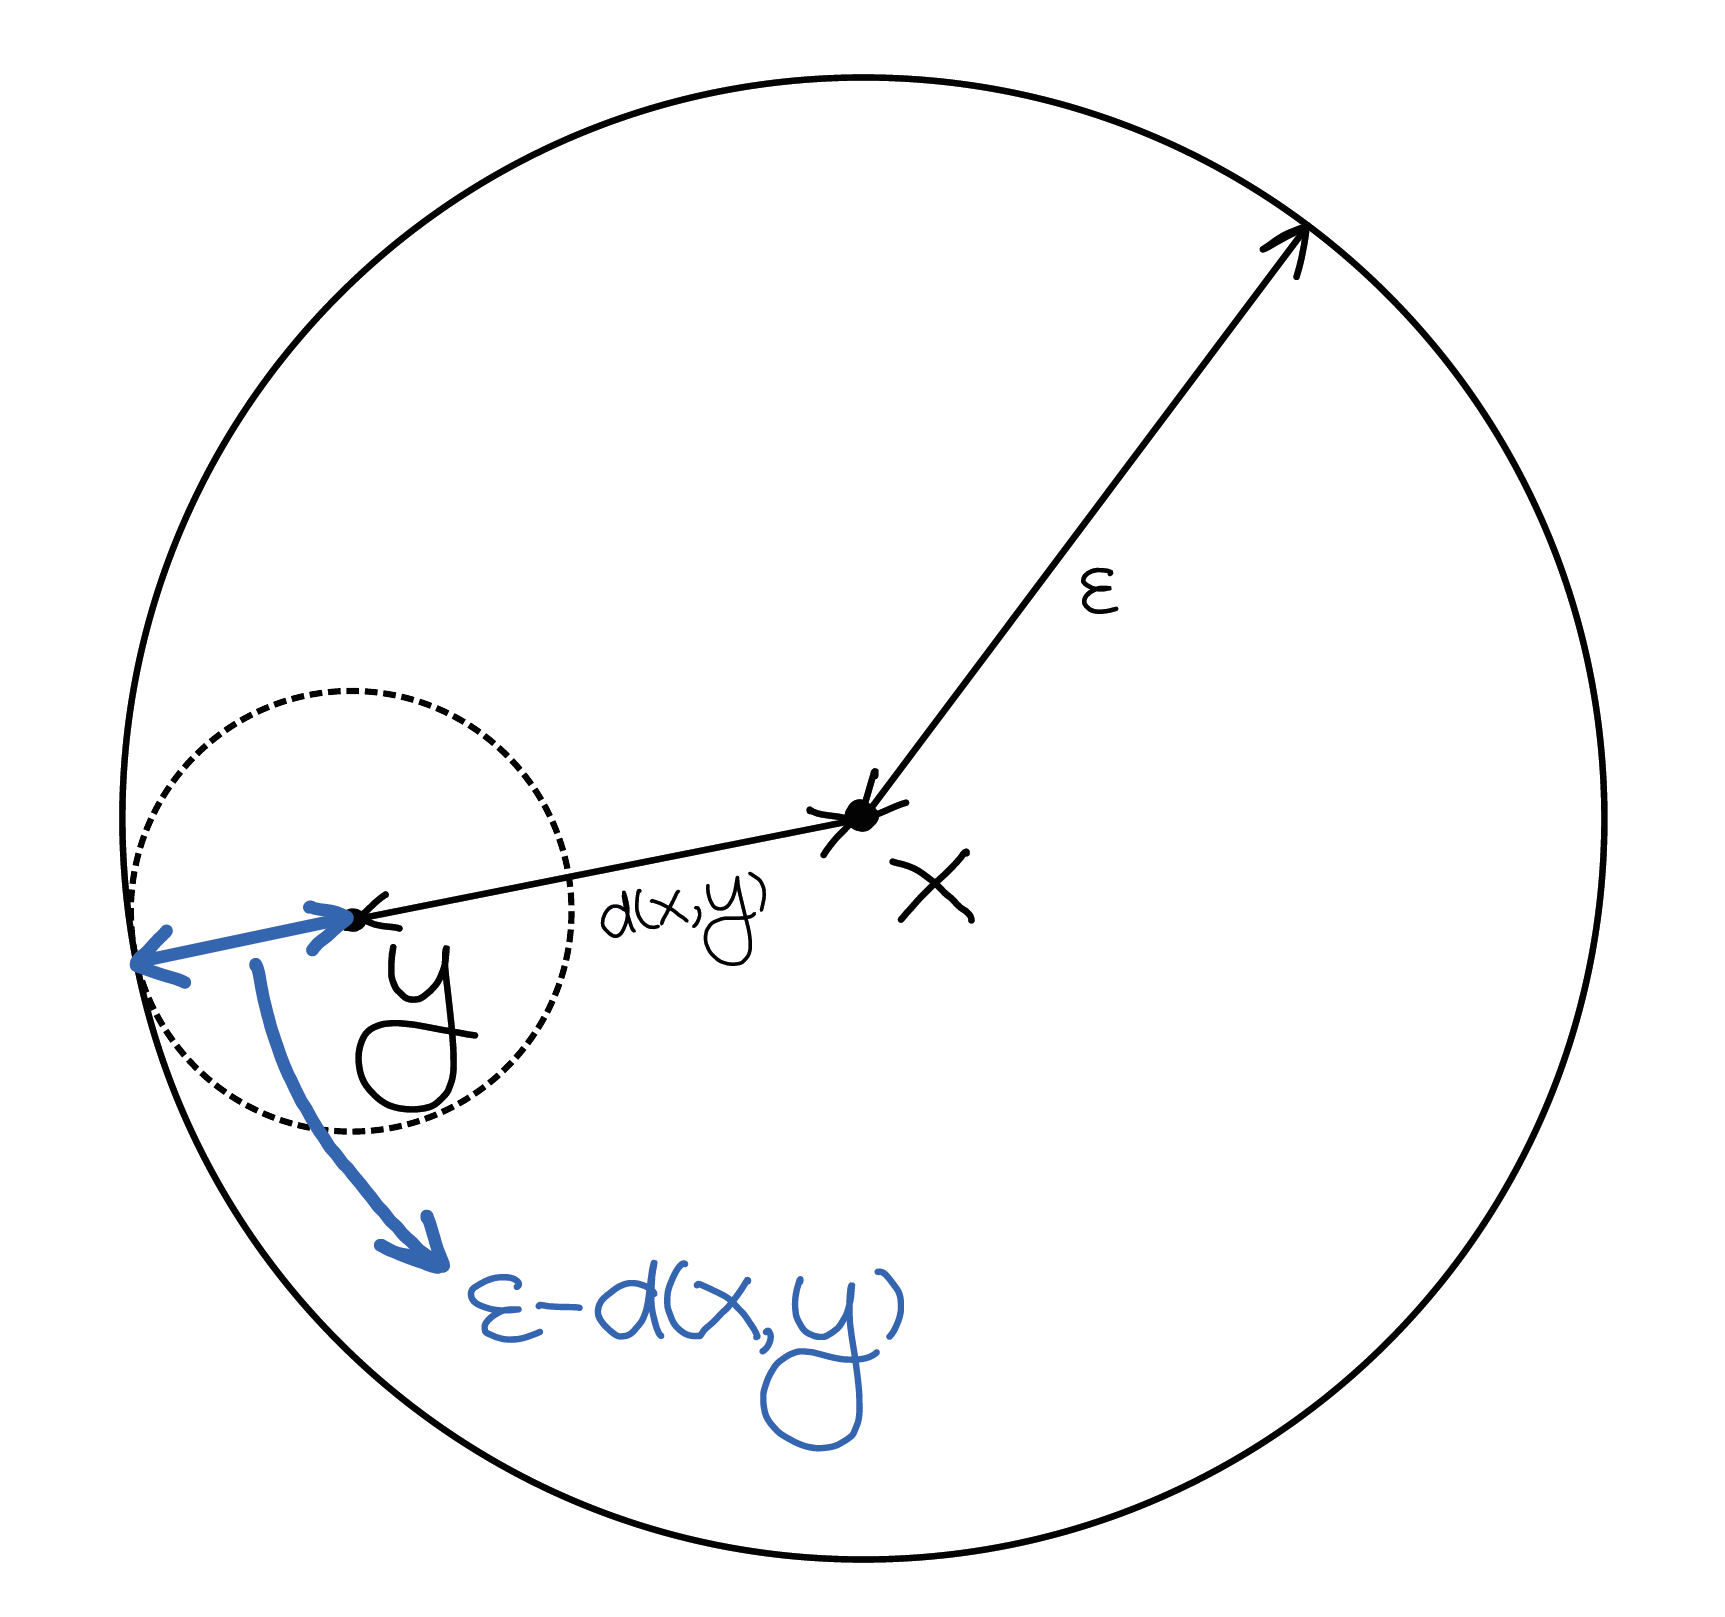
\includegraphics[width=0.6\columnwidth]{week_09_open_ball}
  \caption{Open balls\label{fig:week_09_open_balls}}
\end{figure}
\begin{prop}
  Any open set can be written as a union of open balls.
\end{prop}
\begin{proof}
  Take any open set $A \subseteq X$. Since $A$ is open in $X$, for every $x \in A$, there exists $\epsilon_x > 0$ such that
  \[
    B(x, \epsilon_x) \subseteq A
  \]
  Since this holds for every $x$,
  \[
    \bigcup_{x \in A} B(x, \epsilon_x) \subseteq A
  \]
  For the other direction, take $x \in A$. Then
  \[
    x \in B(x, \epsilon_x) \subseteq \bigcup_{x \in A} B(x, \epsilon_x)
  \]
  Since this is true for every $x \in A$, $A \subseteq \bigcup_{x \in A} B(x, \epsilon_x)$. Therefore, $A = \bigcup_{x \in A} B(x, \epsilon_x)$.
\end{proof}

% ==================================================================================================

\section{Closed sets}
This is one definition of closed sets:
\begin{definition}[Closed set]
  Let $A \subseteq X$. We say that $A$ is closed if $X \backslash A \coloneqq A ^ c$ is open in $X$, where $A ^ c$ is the complement of $A$.
\end{definition}
The complement of $A$ is represented here as $A ^ c$, whereas in discrete maths (COMP40018), it is represented by $\overline{A}$. They are merely notational differences, but since the former is used in the \href{https://web.mit.edu/paigeb/www/18.S097/}{notes} on which this chapter is mostly based, I will stick with $A ^ c$ for my own sanity.
\begin{theorem}
  Let $X$ be a metric space, and let $\{A_i\}_{i \in \Lambda}$ be closed sets in $X$.
  \begin{enumerate}
    \item $\varnothing$ and $X$ are closed sets in $X$.
    \item $\bigcap_{i \in I} A_i$ is closed in $X$. (The arbitrary intersection of closed sets is closed.)
    \item $\bigcup_{i = 1}^n A_i$ is closed in $X$. (The finite union of closed sets is closed.)
  \end{enumerate}
\end{theorem}
To prove the second and third item, we will need De Morgan's Laws for sets:
\begin{theorem}[De Morgan's]
  Consider the sets $\{A_i\}_{i \in \Lambda}$ Then
  \[
    {\left(\bigcup_{i \in \Lambda} A_i \right)} ^ c = \bigcap_{i \in \Lambda} A_i^c \qquad \text{and} \qquad {\left(\bigcap_{i \in \Lambda} A_i \right)} ^ c = \bigcup_{i \in \Lambda} A_i^c
  \]
\end{theorem}
\begin{proof}
  1. The complement of $\varnothing$ is $\varnothing ^ c = X$, which is open, so $\varnothing$ is closed. Similarly, $X ^ c = \varnothing$, so $X$ is closed. Note that $\varnothing$ and $X$ are open and closed at the same time, so these two properties are not mutually exclusive.

  2. We want to show that 
  \[
    {\left(\bigcap_{i \in I} A_i\right)} ^ c = \bigcup_{i \in \Lambda} A_i^c
  \]
  is open. Since $A_i$ is closed for every $i \in \Lambda$, $A_i^c$ is open by definition. From \Cref{thm:topological-prop-open-sets}, we know that the arbitrary union of open sets is open.
  
  3. We want to show that
  \[
    {\left(\bigcup_{i = 1}^n A_i \right)} ^ c = \bigcap_{i = 1}^n A_i^c
  \]
  is open. Since $A_i$ is closed for every $1 \leq i \leq n$, $A_i^c$ is open by definition. From \Cref{thm:topological-prop-open-sets}, we know that the finite intersection of open sets is open.
\end{proof}
\begin{prop}
  Let $(X, d)$ be a metric space, and $x \in X$. Then $\{x\}$ is a closed set in $X$.
\end{prop}
\begin{proof}
  We want to show that $Y \coloneqq X \backslash \{x\}$ is open, and to show that $Y$ is open, for every $y \in Y$, there must exist $\epsilon > 0$ such that
  \[
    B(y, \epsilon) \subseteq Y
  \]
  Take $y \in Y$, and let $\epsilon = d(x, y)$. (To be extra intentional, we can let $\epsilon = d(x, y) / 2$ instead.) We know that $d(x, y) \neq 0$ since $x \notin Y$, and so $x \neq y \in Y$; then $d(x, y) > 0$ follows by positive definiteness. Since $d(x, y)$ is not strictly less than $\epsilon$, $x \notin B(y, \epsilon)$, so it follows that $B(y, \epsilon) \subseteq Y$. 
\end{proof}
We can prove that any finite set is closed in a similar manner. For any finite subset $A = \{x_1, x_2, \ldots, x_n\} \subseteq X$, we simply let $\epsilon = \min_{1 \leq i \leq n} d(x_i, y) = \min\{d(x_1, y), d(x_2, y), \ldots, d(x_n, y)\}$ instead.

The following is an alternative definition of closed sets, which we will show is equivalent to our previous definition.
\begin{prop}[PSET 2, Q2]
  Let $(X, d)$ be a metric space. A subset $A \subseteq X$ is closed if and only if every convergent sequence in $A$ converges in $A$.
\end{prop}
\begin{proof}
  Suppose $A \subseteq X$ is closed. Then $A ^ c$ is open. Take any convergent sequence $x_n$ in $A$ (so $x_n \in A$ for every $n \in \N$), and suppose towards a contradiction that it converges to some $x \notin A$, i.e. $x \in A ^ c$. Since $A ^ c$ is open, there exists $\epsilon > 0$ such that $B(x, \epsilon) \subseteq A ^ c$. However, for this $\epsilon$, since $x_n \to x$, there exists $N \in \N$ such that for all $n > N$, $d(x_n, x) < \epsilon$. So $x_n \in B(x, \epsilon) \subseteq A ^ c$, which contradicts that $x_n$ is a sequence in $A$.

  Now suppose every convergent sequence in $A$ converges in $A$. Suppose, towards a contradiction, that $A ^ c$ is not open. Then there exists $y \in A ^ c$ such that for every $\epsilon > 0$, $B(y, \epsilon) \not\subseteq A ^ c$. Since $B(y, \epsilon) \not\subseteq A ^ c$, this means there exists $x \in B(y, \epsilon)$ such that $x \notin A ^ c$, so $x \in A$. We build a sequence $x_n$ by taking $x_n \in B(y, 1 / n)$ such that $x_n \in A$. Since $1 / n \to 0$, it follows that $d(x_n, y) \to 0$, so $x_n \to y$. However, $x_n$ is a convergent sequence in $A$ and $y \notin A$, contradiction.
\end{proof}

% ==================================================================================================

\section{Neighbourhoods}
There are several different definitions of neighbourhoods. We will adopt the definition on \href{https://en.wikipedia.org/wiki/Neighbourhood_(mathematics)#In_a_metric_space}{Wikipedia} here:
\begin{definition}[Neighbourhood]
  Let $(X, d)$ be a metric space. A set $U$ is a neighbourhood of a point $x \in X$ if there exists $\epsilon > 0$ such that 
  \[
    B(x, \epsilon) \coloneqq \{y \in X \; | \; d(x, y) < \epsilon \} \subseteq U
  \]
  Naturally, from this definition, $x \in B(x, \epsilon) \subseteq U$, but other definitions (especially those concerning more general spaces than metric spaces) will specify that $x \in U$ as a requirement. An \textit{open neighbourhood} is a neighbourhood which is also an open set.
\end{definition}
\begin{prop}
  Let $\{x_n\}$ be a sequence in the metric space $(X, d)$. Then, $x_n$ converges to $x \in X$ if and only if for every neighbourhood of $x$, all but finitely many terms in $x_n$ are in the neighbourhood of $x$.
\end{prop}
\begin{proof}
  Suppose $x_n \to x$ and take some arbitrary neighbourhood $U$ of $x$. Then there exists $\epsilon > 0$ such that $B(x, \epsilon) \subseteq U$. For this $\epsilon$, there exists $N \in \N$ such that $d(x_n, x) < \epsilon$ for every $n > N$, and therefore, $x_n \in B(x, \epsilon)$. There can only be finitely many terms (including and up to $x_N$, but not necessarily all of them) that are not in $B(x, \epsilon)$, so all but finitely many terms are in $B(x, \epsilon) \subseteq U$.

  Now take an arbitrary $\epsilon > 0$. The ball $B(x, \epsilon)$ is a neighbourhood of $x$. Suppose all but finitely many terms in $x_n$ are in $B(x, \epsilon)$. Let $x_N$ denote the last term that is not in the ball. (If no such term exists, then we are done.) Then for every $n > N$, $x_n \in B(x, \epsilon)$.
\end{proof}

% ==================================================================================================

\section{Continuous functions}
We will show how continuous functions tie up the previous sections.
\begin{prop}
  Let $(X, d_X)$ and $(Y, d_Y)$ be metric spaces. Then $f: X \to Y$ is continuous at $c \in X$ if and only if for every sequence $\{x_n\}$ in $X$ converging to $c$, $f(x_n) \to f(c)$.
\end{prop}
\begin{proof}
  Suppose $f$ is continuous at $c$, and take any sequence $\{x_n\}$ in $X$ that converges to $c$. We want to show that
  \[
    \forall \epsilon > 0, \; \exists N \in \N: n > N \implies d_Y(f(x_n), f(c)) < \epsilon
  \]
  Given that $x_n \to c$, we have
  \[
    \forall \epsilon > 0, \; \exists N \in \N: n > N \implies d_X(x_n, c) < \epsilon
  \]
  and given $f$ continuous at $c$, we have for every $x \in X$,
  \[
    \forall \epsilon > 0, \; \exists \delta > 0: d_X(x, c) < \delta \implies d_Y(x, c) < \epsilon
  \]
  Fix $\epsilon > 0$. For this $\delta > 0$, by $x_n \to c$, we have
  \[
    \exists N \in \N: n > N \implies d_X(x_n, c) < \delta
  \]
  Therefore, by continuity of $f$, we have $d_Y(x_n, c) < \epsilon$ for every $n > N$, as required.

  Now suppose $f$ is not continuous at $c$. We want to find a sequence $\{x_n\}$ such that $x_n \to c$ but $f(x_n) \not\to f(c)$. Given that $f$ is not continuous at $c$,
  \[
    \exists \epsilon > 0: \forall \delta > 0, \; \exists x \in X: d_X(x, c) < \delta \land d_Y(f(x), f(c)) \geq \epsilon
  \]
  Whenever we see $\forall \delta > 0$, think of $1 / n$. For this $\epsilon > 0$, we can construct a sequence $x_n$ satisfying
  \[
    d_X(x_n, c) < \frac{1}{n} \qquad \text{and} \qquad d_Y(f(x_n), f(c)) \geq \epsilon > 0
  \]
  By squeeze theorem, $d_X(x_n, c) \to 0$, so $x_n \to c$. However, $d_Y(f(x_n), f(c)) \not\to 0$, so $f(x_n) \not\to f(c)$.
\end{proof}
\begin{prop}
  Let $(X, d_X)$ and $(Y, d_Y)$ be metric spaces. Then $f: X \to Y$ is continuous at $c \in X$ if and only if for every open neighbourhood $U$ of $f(c)$ in $Y$, the set $f ^ {-1} (U)$ contains an open neighbourhood of $c$ in $X$.
\end{prop}
\begin{proof}
  Suppose $f$ is continuous at $c$, and let $U$ be an open neighbourhood of $f(c)$. We want to find some $\epsilon > 0$ such that
  \[
    B(c, \epsilon) \subseteq f ^ {-1} (U)
  \]
  Given $f$ is continuous at $c$, for every $x \in X$,
  \[
    \forall \epsilon > 0, \; \exists \delta > 0: d_X(x, c) < \delta \implies d_Y(f(x), f(c)) < \epsilon
  \]
  and given $U$ is open in $Y$, there exists $\epsilon > 0$ such that 
  \[
    B(f(c), \epsilon) \coloneqq \{y \in Y \; | \; d(y, f(c)) < \epsilon \} \subseteq U
  \]
  For this $\epsilon$, by continuity of $f$ at $c$, there exists $\delta > 0$ such that for every $x \in X$,
  \[
    d_X(x, c) < \delta \implies d_Y(f(x), f(c)) < \epsilon
  \]
  In other words, for every $x \in X$,
  \[
    x \in B(c, \delta) \implies f(x) \in B(f(c), \epsilon)
  \]
  Since $x \in f ^ {-1} (f(x))$ ($f ^ {-1}$ returns the preimage of its argument, which is a set in general), it follows that
  \[
    B(c, \delta) \subseteq f ^ {-1} (B(f(c), \epsilon)) \subseteq f ^ {-1} (U)
  \]

  Now suppose for every open neighbourhood $U$ of $f(c)$, $f ^ {-1} (U)$ contains an open neighbourhood of $c$. We want to show that for every $x \in X$,
  \[
    \forall \epsilon > 0, \; \exists \delta > 0: d_X(x, c) < \delta \implies d_Y(f(x), f(c)) < \epsilon
  \]
  Fix $\epsilon > 0$, and consider $U = B(f(c), \epsilon)$. It is clearly an open neighbourhood of $f(c)$. Then $f ^ {-1} (U)$ contains an open neighbourhood $V$ of $c$. By our definition of neighbourhoods, there exists $\delta > 0$ such that
  \[
    B(c, \delta) \subseteq V \subseteq f ^ {-1} (U)
  \]
  (An irrelevant but noteworthy point: we don't know if $f ^ {-1} (U)$ is open, but it is given that $V$ is open.) In other words, for every $x \in X$,
  \[
    x \in B(c, \delta) \implies x \in f ^ {-1} (U)
  \]
  and therefore,
  \[
    x \in B(c, \delta) \implies f(x) \in U = B(f(c), \epsilon)
  \]
\end{proof}
\begin{prop}[PSET 2, Q7]
  Let $(X, d_X)$ and $(Y, d_Y)$ be metric spaces. Then $f: X \to Y$ is continuous if and only if for every set $U$ open in $Y$, $f ^ {-1} (U)$ is open in $X$.
\end{prop}
\begin{proof}
  Suppose $f$ is continuous. Then for every $c \in X$ we have
  \[
    \forall \epsilon > 0, \; \exists \delta > 0: d_X(x, c) < \delta \implies d_Y(f(x), f(c)) < \epsilon 
  \]
  Take any set $U$ open in $Y$. We want to show that for every $x \in f ^ {-1} (U)$, there exists $\epsilon > 0$ such that
  \[
    B(x, \epsilon) \subseteq f ^ {-1} (U)
  \]
  Since $U$ is open, for every $y \in Y$, there exists $\epsilon > 0$ such that
  \[
    B(y, \epsilon) \subseteq U
  \]
  For every $x \in f ^ {-1} (U)$, $f(x) \in U$. So there exists $\epsilon > 0$ such that
  \[
    B(f(x), \epsilon) \subseteq U
  \]
  Fix $x_0 \in X$. Then there exists $\epsilon > 0$ such that $B(f(x_0), \epsilon) \subseteq U$. Since $f$ is continuous, there exists $\delta > 0$ such that for every $x \in X$,
  \[
    x \in B(x_0, \delta) \implies f(x) \in B(f(x_0), \epsilon) \subseteq U
  \]
  so
  \[
    x \in B(x_0, \delta) \implies x \in f ^ {-1} (U)
  \]
  and therefore,
  \[
    B(x_0, \delta) \subseteq f ^ {-1} (U)
  \]
  This holds for every $x_0 \in X$, so $f ^ {-1} (U)$ is open, as required.

  Now suppose for every set $U$ open in $Y$, $f ^ {-1} (U)$ is open in $X$. We want to show that for every $c \in X$ and every $\epsilon > 0$,
  \[
    \exists \delta > 0: d_X(x, c) < \delta \implies d_Y(f(x), f(c)) < \epsilon
  \]
  Fix $c \in X$ and $\epsilon > 0$. Let $U = B(f(c), \epsilon)$. It is clearly open in $Y$. ($f(c)$ exists since $f$ is a function.) So $f ^ {-1} (U)$ is open in $X$. In particular, since $f(c) \in U$, it follows that $c \in f ^ {-1} (U)$. The rest follows exactly as the sufficient direction of the previous proof. Since $\epsilon > 0$ is arbitrary, $f$ is continuous at $c$. Since $c \in X$ is arbitrary, $f$ is continuous.
\end{proof}